% Options for packages loaded elsewhere
\PassOptionsToPackage{unicode,linktoc=all}{hyperref}
\PassOptionsToPackage{hyphens}{url}
\PassOptionsToPackage{dvipsnames,svgnames,x11names}{xcolor}
%
\documentclass[
  a4paper,
]{article}
\usepackage{amsmath,amssymb}
\usepackage{iftex}
\ifPDFTeX
  \usepackage[T1]{fontenc}
  \usepackage[utf8]{inputenc}
  \usepackage{textcomp} % provide euro and other symbols
\else % if luatex or xetex
  \usepackage{unicode-math} % this also loads fontspec
  \defaultfontfeatures{Scale=MatchLowercase}
  \defaultfontfeatures[\rmfamily]{Ligatures=TeX,Scale=1}
\fi
\usepackage{lmodern}
\ifPDFTeX\else
  % xetex/luatex font selection
\fi
% Use upquote if available, for straight quotes in verbatim environments
\IfFileExists{upquote.sty}{\usepackage{upquote}}{}
\IfFileExists{microtype.sty}{% use microtype if available
  \usepackage[]{microtype}
  \UseMicrotypeSet[protrusion]{basicmath} % disable protrusion for tt fonts
}{}
\makeatletter
\@ifundefined{KOMAClassName}{% if non-KOMA class
  \IfFileExists{parskip.sty}{%
    \usepackage{parskip}
  }{% else
    \setlength{\parindent}{0pt}
    \setlength{\parskip}{6pt plus 2pt minus 1pt}}
}{% if KOMA class
  \KOMAoptions{parskip=half}}
\makeatother
\usepackage{xcolor}
\usepackage[margin=25mm]{geometry}
\usepackage{longtable,booktabs,array}
\usepackage{calc} % for calculating minipage widths
% Correct order of tables after \paragraph or \subparagraph
\usepackage{etoolbox}
\makeatletter
\patchcmd\longtable{\par}{\if@noskipsec\mbox{}\fi\par}{}{}
\makeatother
% Allow footnotes in longtable head/foot
\IfFileExists{footnotehyper.sty}{\usepackage{footnotehyper}}{\usepackage{footnote}}
\makesavenoteenv{longtable}
\usepackage{graphicx}
\makeatletter
\def\maxwidth{\ifdim\Gin@nat@width>\linewidth\linewidth\else\Gin@nat@width\fi}
\def\maxheight{\ifdim\Gin@nat@height>\textheight\textheight\else\Gin@nat@height\fi}
\makeatother
% Scale images if necessary, so that they will not overflow the page
% margins by default, and it is still possible to overwrite the defaults
% using explicit options in \includegraphics[width, height, ...]{}
\setkeys{Gin}{width=\maxwidth,height=\maxheight,keepaspectratio}
% Set default figure placement to htbp
\makeatletter
\def\fps@figure{htbp}
\makeatother
\setlength{\emergencystretch}{3em} % prevent overfull lines
\providecommand{\tightlist}{%
  \setlength{\itemsep}{0pt}\setlength{\parskip}{0pt}}
\setcounter{secnumdepth}{-\maxdimen} % remove section numbering
\newlength{\cslhangindent}
\setlength{\cslhangindent}{1.5em}
\newlength{\csllabelwidth}
\setlength{\csllabelwidth}{3em}
\newlength{\cslentryspacingunit} % times entry-spacing
\setlength{\cslentryspacingunit}{\parskip}
\newenvironment{CSLReferences}[2] % #1 hanging-ident, #2 entry spacing
 {% don't indent paragraphs
  \setlength{\parindent}{0pt}
  % turn on hanging indent if param 1 is 1
  \ifodd #1
  \let\oldpar\par
  \def\par{\hangindent=\cslhangindent\oldpar}
  \fi
  % set entry spacing
  \setlength{\parskip}{#2\cslentryspacingunit}
 }%
 {}
\usepackage{calc}
\newcommand{\CSLBlock}[1]{#1\hfill\break}
\newcommand{\CSLLeftMargin}[1]{\parbox[t]{\csllabelwidth}{#1}}
\newcommand{\CSLRightInline}[1]{\parbox[t]{\linewidth - \csllabelwidth}{#1}\break}
\newcommand{\CSLIndent}[1]{\hspace{\cslhangindent}#1}
\ifLuaTeX
\usepackage[bidi=basic]{babel}
\else
\usepackage[bidi=default]{babel}
\fi
\babelprovide[main,import]{british}
% get rid of language-specific shorthands (see #6817):
\let\LanguageShortHands\languageshorthands
\def\languageshorthands#1{}
% $HOME/.pandoc/defaults/latex-header-includes.tex
% Common header includes for both lualatex and xelatex engines.
%
% Preliminaries
%
% \PassOptionsToPackage{rgb,dvipsnames,svgnames}{xcolor}
% \PassOptionsToPackage{main=british}{babel}
\PassOptionsToPackage{english}{selnolig}
\AtBeginEnvironment{quote}{\small}
\AtBeginEnvironment{quotation}{\small}
\AtBeginEnvironment{longtable}{\centering}
%
% Packages that are useful to include
%
\usepackage{graphicx}
\usepackage{subcaption}
\usepackage[inkscapeversion=1]{svg}
\usepackage[defaultlines=4,all]{nowidow}
\usepackage{etoolbox}
\usepackage{fontsize}
\usepackage{newunicodechar}
\usepackage{pdflscape}
\usepackage{fnpct}
\usepackage{parskip}
  \setlength{\parindent}{0pt}
\usepackage[style=american]{csquotes}
% \usepackage{setspace} Use the <fontname-plus.tex> files for setspace
%
\usepackage{esdiff} % for derivative symbols
\usepackage{amsmath}
\usepackage{hyperref} % cleveref must come AFTER hyperref
\usepackage[capitalize,noabbrev]{cleveref} % Must come after hyperref
% noto-plus.tex
% Font-setting header file for use with Pandoc Markdown
% to generate PDF via LuaLaTeX.
% The main font is Noto Serif.
% Other main fonts are also available in appropriately named file.
\usepackage{fontspec}
\usepackage{setspace}
\setstretch{1.3}
%
\defaultfontfeatures{Ligatures=TeX,Scale=MatchLowercase,Renderer=Node} % at the start always
%
% For English
% See also https://tex.stackexchange.com/questions/574047/lualatex-amsthm-polyglossia-charissil-error
% We use Node as Renderer for the Latin Font and Greek Font and HarfBuzz as renderer ofr Indic fonts.
%
\babelfont{rm}[Script=Latin,Scale=1]{NotoSerif}% Config is at $HOME/texmf/tex/latex/NotoSerif.fontspec
%
\babelfont{sf}[Script=Latin]{SourceSansPro}% Config is at $HOME/texmf/tex/latex/SourceSansPro.fontspec
%
\babelfont{tt}[Script=Latin]{FiraMono}% Config is at $HOME/texmf/tex/latex/FiraMono.fontspec
%
% Sanskrit, Tamil, and Greek fonts
%
\babelprovide[import, onchar=ids fonts]{sanskrit}
\babelprovide[import, onchar=ids fonts]{tamil}
\babelprovide[import, onchar=ids fonts]{greek}
%
\babelfont[sanskrit]{rm}[Scale=1.1,Renderer=HarfBuzz,Script=Devanagari]{NotoSerifDevanagari}
\babelfont[sanskrit]{sf}[Scale=1.1,Renderer=HarfBuzz,Script=Devanagari]{NotoSansDevanagari}
\babelfont[tamil]{rm}[Renderer=HarfBuzz,Script=Tamil]{NotoSerifTamil}
\babelfont[tamil]{sf}[Renderer=HarfBuzz,Script=Tamil]{NotoSansTamil}
\babelfont[greek]{rm}[Script=Greek]{GentiumBookPlus}
%
% Math font
%
\usepackage{unicode-math} % seems not to hurt % fallabck
\setmathfont[bold-style=TeX]{STIX Two Math}
%
%
% Other fonts
%
\newfontfamily{\emojifont}{Symbola}
%

\usepackage{titling}
\usepackage{fancyhdr}
    \pagestyle{fancy}
    \fancyhead{}
    \fancyfoot{}
    \renewcommand{\headrulewidth}{0.2pt}
    \renewcommand{\footrulewidth}{0.2pt}
    \fancyhead[LO,RE]{\scshape\thetitle}
    \fancyfoot[CO,CE]{\footnotesize Copyright © 2006\textendash\the\year, R (Chandra) Chandrasekhar}
    \fancyfoot[RE,RO]{\thepage}
\newfontfamily{\regulariconfont}{Font Awesome 6 Free Regular}[Color=Grey]
\newfontfamily{\solidiconfont}{Font Awesome 6 Free Solid}[Color=Grey]
\newfontfamily{\brandsiconfont}{Font Awesome 6 Brands}[Color=Grey]
%
% Direct input of Unicode code points
%
\newcommand{\faEnvelope}{\regulariconfont\ ^^^^f0e0\normalfont}
\newcommand{\faMobile}{\solidiconfont\ ^^^^f3cd\normalfont}
\newcommand{\faLinkedin}{\brandsiconfont\ ^^^^f0e1\normalfont}
\newcommand{\faGithub}{\brandsiconfont\ ^^^^f09b\normalfont}
\newcommand{\faAtom}{\solidiconfont\ ^^^^f5d2\normalfont}
\newcommand{\faPaperPlaneRegular}{\regulariconfont\ ^^^^f1d8\normalfont}
\newcommand{\faPaperPlaneSolid}{\solidiconfont\ ^^^^f1d8\normalfont}

%
% The block below is commented out because of Tofu glyphs in HTML
%
% \newcommand{\faEnvelope}{\regulariconfont\ \normalfont}
% \newcommand{\faMobile}{\solidiconfont\ \normalfont}
% \newcommand{\faLinkedin}{\brandsiconfont\ \normalfont}
% \newcommand{\faGithub}{\brandsiconfont\ \normalfont}
\ifLuaTeX
  \usepackage{selnolig}  % disable illegal ligatures
\fi
\IfFileExists{bookmark.sty}{\usepackage{bookmark}}{\usepackage{hyperref}}
\IfFileExists{xurl.sty}{\usepackage{xurl}}{} % add URL line breaks if available
\urlstyle{sf}
\hypersetup{
  pdftitle={The Two Most Important Numbers: Zero and One},
  pdfauthor={R (Chandra) Chandrasekhar},
  pdflang={en-GB},
  colorlinks=true,
  linkcolor={DarkOliveGreen},
  filecolor={Purple},
  citecolor={DarkKhaki},
  urlcolor={Maroon},
  pdfcreator={LaTeX via pandoc}}

\title{The Two Most Important Numbers: Zero and One}
\author{R (Chandra) Chandrasekhar}
\date{2023-10-31 | 2023-11-01}

\begin{document}
\maketitle

\thispagestyle{empty}


The unique properties of the numbers zero and one make them
mathematically interesting and indispensable. In this slow-paced stroll
though the ideas streaming out of these two numbers, we uncover
well-known as well as relatively obscure facts about them. It is hoped
that in the process we may discover how they cement together disparate
areas of Mathematics.

\hypertarget{starting-at-the-beginning}{%
\subsection{Starting at the beginning}\label{starting-at-the-beginning}}

At first, I thought I would skirt around the formal sets of numbers, and
concepts like commutativity and associativity, and keep this blog very
informal. But I found that each time I tried that approach, I would have
to furtively sneak in a paragraph here, or a footnote there, as
explanation of these ideas. In the end, I decided to start at the
beginning, and work my way through the natural numbers, the integers,
the rationals, etc., and
\href{https://www.thefreedictionary.com/broach}{broach} ideas like
commutativity and associativity.

\hypertarget{counting}{%
\subsection{Counting}\label{counting}}

Aeons ago, a shepherd with five sheep might have counted, ``one sheep,
two sheep, three sheep, four sheep, and five sheep.'' But wait! Since he
did not have the names for numbers---nor indeed the abstract concept of
a number---he could not have done that. So, what did he do? Let us
speculate.

\hypertarget{naming-sheep}{%
\subsubsection{Naming sheep}\label{naming-sheep}}

He could have given \emph{unique} names to each of his five sheep and
developed enough familiarity with them to identify them by name. Then
all he needed to do was to check that all his named sheep were home by
sundown. But such a method would have become cumbersome and error-prone
as his flock multiplied.

\hypertarget{one-to-one-correspondence}{%
\subsubsection{One-to-one
correspondence}\label{one-to-one-correspondence}}

The later, and more likely, alternative was to use stones to correspond
to sheep. He could have taken a leather bag and dropped a stone in
it---one for each sheep that he owned. He did not need to learn
counting. All he needed to do was to establish a
\href{https://www.encyclopedia.com/science/encyclopedias-almanacs-transcripts-and-maps/one-one-correspondence}{one-to-one
correspondence}\footnote{One-to-one correspondence is a simple but
  extremely powerful idea which guided
  \href{https://www.britannica.com/science/one-to-one-correspondence}{Georg
  Cantor} to develop his radical but consistent ideas about types of
  infinity.} between sheep and stone. As long as he had the right number
of stones in his bag, he could account for each one of his sheep.

The Latin word for \emph{stone} is
\href{https://www.etymonline.com/search?q=calculus}{calculus}, and from
the stone has come the whole science of \emph{calculation}.

\hypertarget{measurement}{%
\subsection{Measurement}\label{measurement}}

When we \emph{count}, as with sheep, where do we start? We start with
one. We do not start with zero, because we cannot point to any sheep or
other object and say ``zero''.

Nevertheless, zero has fundamental importance when we start
\emph{measuring}. When the petrol tank in a car is empty, we can fill it
up and measure the volume of petrol for which we have to pay.

When we count, we start with \(1\).

When we measure, we start with \(0\).

\hypertarget{sets-of-numbers}{%
\subsection{Sets of numbers}\label{sets-of-numbers}}

Although Mathematics has rigorous foundations, at the very bottom, its
notions are not defined
\href{https://www.vocabulary.com/dictionary/explicitly}{explicitly}. One
such notion is that of a \emph{set}, which is loosely defined as a
collection of objects that can either be enumerated or described
clearly. The \emph{sets of numbers} we will deal with have names,
symbols, and definitions as shown below.

\begin{footnotesize}

\begin{longtable}[]{@{}
  >{\raggedright\arraybackslash}p{(\columnwidth - 4\tabcolsep) * \real{0.3457}}
  >{\centering\arraybackslash}p{(\columnwidth - 4\tabcolsep) * \real{0.0370}}
  >{\raggedright\arraybackslash}p{(\columnwidth - 4\tabcolsep) * \real{0.6173}}@{}}
\toprule\noalign{}
\begin{minipage}[b]{\linewidth}\raggedright
Name
\end{minipage} & \begin{minipage}[b]{\linewidth}\centering
Symbol
\end{minipage} & \begin{minipage}[b]{\linewidth}\raggedright
Definition
\end{minipage} \\
\midrule\noalign{}
\endhead
\bottomrule\noalign{}
\endlastfoot
Natural numbers & \(\mathbb{N}\) & \(\{1, 2, 3, 4, ...\}\) \\
Integers & \(\mathbb{Z}\) & \(\{... -3, -2, -1, 0, 1, 2, 3, ...\}\) \\
Rational numbers & \(\mathbb{Q}\) &
\(\{x: x = \frac{p}{q} \mbox{ where } p, q \in \mathbb{Z} \mbox{ and } q \ne 0\}\) \\
Irrational numbers & & \(\{\)The numbers which are not rational\(\}\) \\
Real numbers & \(\mathbb{R}\) & \(\{\)The rationals and the
irrationals\(\}\) \\
Complex numbers & \(\mathbb{C}\) &
\(\{a+ib: a, b \in \mathbb{R} \mbox{ and } i^2 = -1\}\) \\
\end{longtable}

\end{footnotesize}

\hfill\break
While it is premature to talk about these sets and their peculiarities
in this blog, it is worth making some points about them.

\begin{enumerate}
\item
  The symbols in the second column are called
  \href{https://oeis.org/wiki/Blackboard_bold}{blackboard bold} letters.
\item
  A set is traditionally enclosed in a pair of \emph{braces}: \(\{\}\).
\item
  There is \href{https://en.wikipedia.org/wiki/Natural_number}{no
  agreement on whether or not to include zero} as a member of
  \(\mathbb{N}\). I have chosen not to because I consider \(\mathbb{N}\)
  the set of \emph{counting numbers}.
\item
  Zero is neither positive nor negative. It is itself and, as a set, is
  often denoted \(\{0\}\).
\item
  The \emph{integers} are named \(\mathbb{Z}\) after the German word
  \emph{Zahlen} which stands for ``numbers'' (singular \emph{Zahl}). The
  integers include positive and negative whole numbers as well as zero.
\item
  The \emph{rational numbers} are so named because they are really
  \emph{ratios} of whole numbers with the proviso that the denominator
  cannot be zero. The symbol \(\mathbb{Q}\) is used because it denotes
  \emph{quotient} the result of \emph{division}.
\item
  There is no symbol for the \emph{irrationals}, which are simply
  defined as numbers which are \emph{not rational}. In fact, the set of
  irrationals may shown, using set notation only indirectly as
  \(\mathbb{R}\setminus\mathbb{Q}\), which means the set of real
  numbers, excluding the rational numbers.
\item
  The \emph{real numbers}, with symbol \(\mathbb{R}\) for real, are
  glibly described as the union of the rational numbers and the
  irrational numbers.\footnote{\href{https://en.wikipedia.org/wiki/Richard_Dedekind}{Richard
    Dedekind} with his \emph{Schnitt} or cut, showed that the rationals
    and irrationals comprise \(\mathbb{R}\), but that is
    \href{https://arpita95b.medium.com/cutting-through-the-confusion-how-dedekind-cuts-build-the-real-numbers-20aeaaec021d}{a
    story} for another day and another blog.}
\item
  The \emph{complex} numbers incorporate a non-real entity called \(i\)
  the \emph{imaginary unit}, which is defined as \(i^2 = -1\). Since
  every real number when squared is greater than or equal to zero, this
  \(i\) is not a real number, and therefore demands its own symbol,
  arithmetic, and set, \(\mathbb{C}\).
\end{enumerate}

\hypertarget{the-four-arithmetic-operations}{%
\subsection{The Four arithmetic
operations}\label{the-four-arithmetic-operations}}

Each of the four basic arithmetic operations--addition, multiplication,
subtraction, division---are
\href{https://en.wikipedia.org/w/index.php?title=Binary_operation\&oldid=1182322931}{binary}
operations and may only be performed between \emph{two} numbers. The
ability to \emph{add} multiple numbers---as in determining the total sum
to be paid at the checkout counter while shopping---is made possible by
the
\href{https://en.wikipedia.org/wiki/Commutative_property}{commutativity}
and
\href{https://en.wikipedia.org/wiki/Associative_property}{associativity}
of addition, which also applies to multiplication. Subtraction and
division are neither commutative nor associative.\footnote{For a start,
  subtraction is not commutative: \(3 - 2 = 1 \ne -1 = 2 - 3\).}

\hypertarget{commutativity-and-associativity}{%
\subsubsection{Commutativity and
Associativity}\label{commutativity-and-associativity}}

Let us add three numbers, \(2\), \(3\), and \(5\). It is common to write
this as \(2 + 3 + 5 = 10\). The sum \(10\) is correct, but its
correctness is derived from the commutativity and associativity of
addition.

In commutativity, we have \[
2 + 3 = 3 + 2.
\] \emph{The order of the two operands may be interchanged}.

In associativity, we have \emph{three operands}. We use parentheses to
denote the operation we perform first. It does not matter which pair we
add first. \[
(2 + 3) + 5 = 2 + (3 + 5).
\] Together, commutativity and associativity allow us to be casual about
the order in which we add several numbers.

Multiplication is repeated addition and it is commutative. Both
properties are easily understood from a geometric demonstration as shown
in \cref{fig:mult}.

\begin{figure}
\hypertarget{fig:mult}{%
\centering
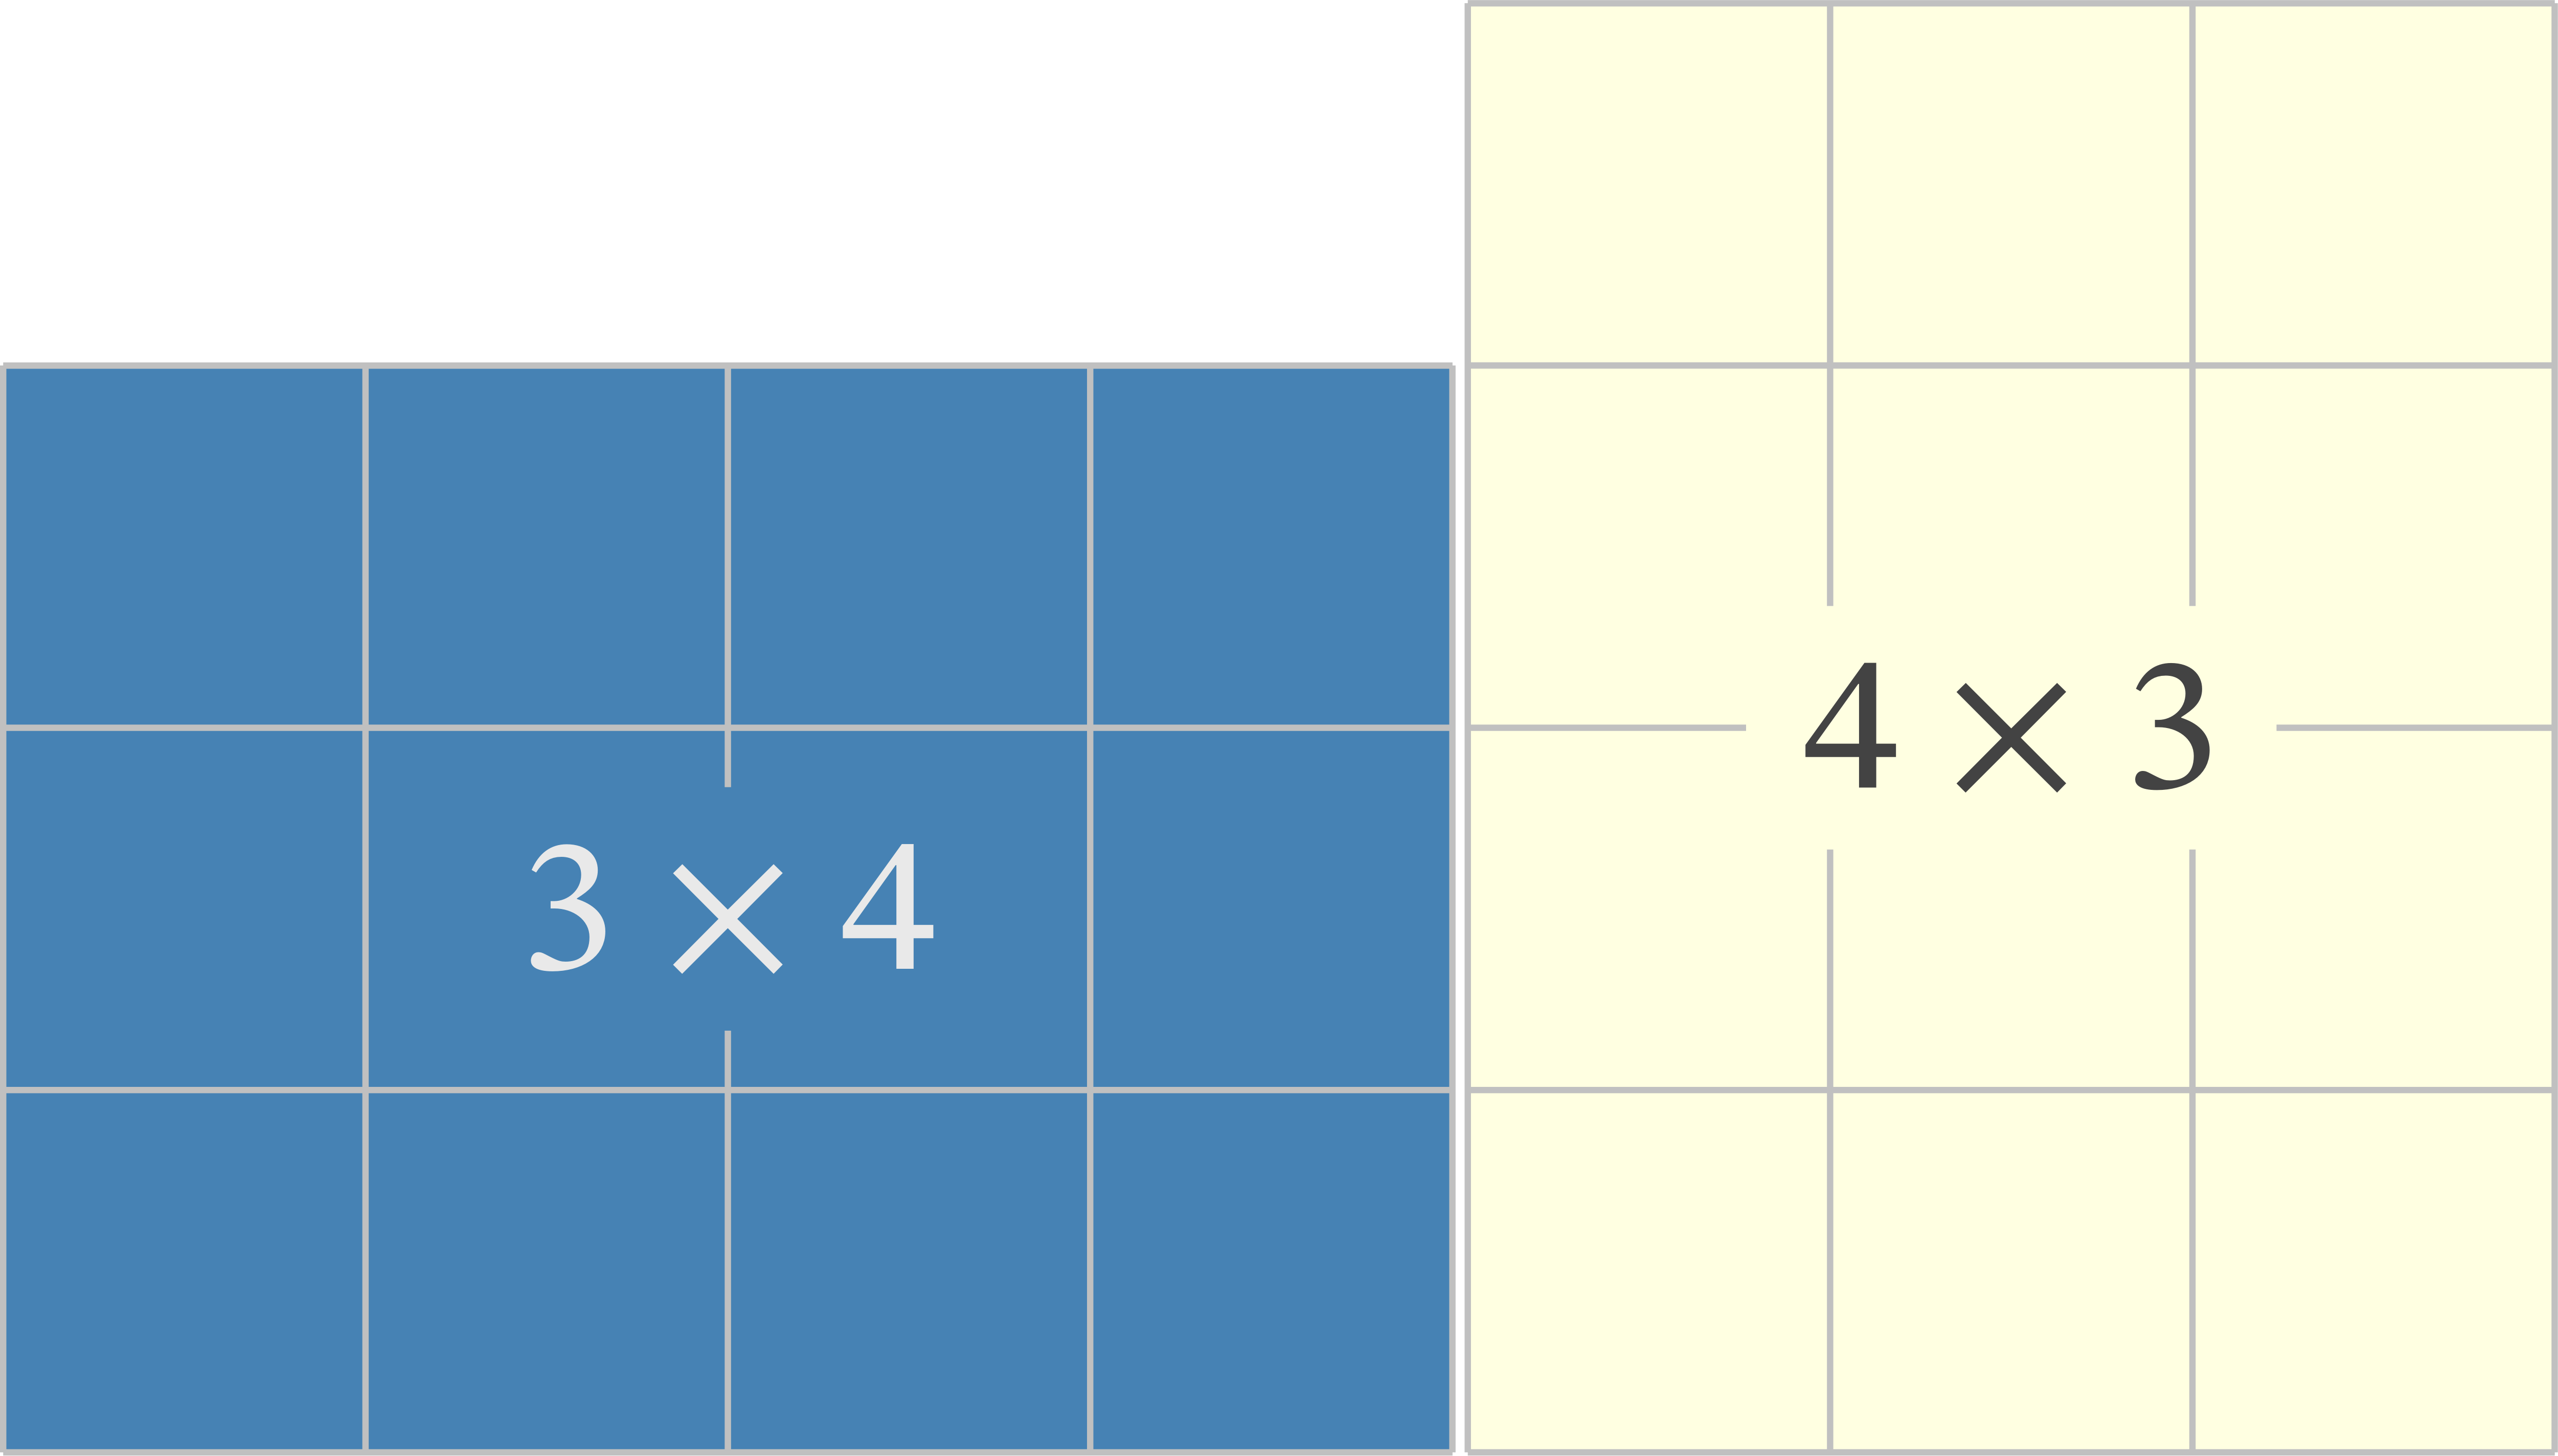
\includegraphics[width=0.6\textwidth,height=\textheight]{images/four-by-three.png}
\caption{The products \(4\times3\) and \(3\times4\) amount to repeated
additions and yield the same result of 12.}\label{fig:mult}
}
\end{figure}

Talking about commutativity and associativity might seem like overkill
for the addition and multiplication of real numbers. But, identifying
these properties is a useful insight, as the more sophisticated
mathematical objects we will encounter later may not obey either or both
properties.

\hypertarget{addition}{%
\subsection{Addition}\label{addition}}

If we start with zero and add one to it, we get one. If we add one to
that we get two. In this fashion, all the natural numbers may be
generated successively by adding one. The \emph{next number} is called
the \emph{successor}. Even if we did not start with zero, but started
with one, instead, we can still generate the entire set \(\mathbb{N}\)
by adding one successively. This method shows that there is no largest
natural number. If there were such a number, say \(p\), we could always
add one to it and show the assumption to be false. In this sense, one
helps us to understand infinity (of the countable variety).

Zero is the \emph{additive identity}, meaning that if we add zero to any
number, the result is the original number again. This means that adding
zero to zero produces zero. Henceforth, let us denote an arbitrary real
number by \(a\), i.e., \(a \in \mathbb{R}\). Then, \[
a + 0 = 0 + a = a.
\]

This is also true of other mathematical objects. The zero of the complex
numbers is \(0 + i(0) = 0\) as well. And adding it to any complex number
also gives us the original complex number.

A \href{https://mathworld.wolfram.com/Matrix.html}{matrix} is
mathematical object which I facetiously call \emph{numbers in teabags}.
They may come in different shapes and sizes. Let us consider a general
\(2\times2\) square matrix like
\(\begin{bmatrix}a & b\\c & d\end{bmatrix}\) which has two horizontal
rows and two vertical columns. The additive identity for this matrix is
a \(2\times2\) square matrix, all of whose entries are zero: \[
\begin{bmatrix}
a & b\\
c & d
\end{bmatrix}
+
\begin{bmatrix}
0 & 0\\
0 & 0
\end{bmatrix}
=
\begin{bmatrix}
a & b\\
c & d
\end{bmatrix}
=
\begin{bmatrix}
0 & 0\\
0 & 0
\end{bmatrix}
+
\begin{bmatrix}
a & b\\
c & d
\end{bmatrix}
\]

\href{https://mathworld.wolfram.com/Polynomial.html}{Polynomials} are
expressions like \(x^2 + 3x + 1\) where \(x\) is some real variable. The
zero polynomial is simply the number zero, and adding it to any
polynomial also gives us back the original polynomial.

\hypertarget{subtraction}{%
\subsection{Subtraction}\label{subtraction}}

Subtracting zero from a number leaves it unchanged. Subtracting a larger
natural number from a smaller one gives a negative number and is the
main reason for expanding the set \(\mathbb{N}\) into the set
\(\mathbb{Z}\).

By convention, when a sign is not prefixed to a number, we assume it to
be positive. If a negative sign is prefixed to a number, it is a
negative number. This is indicated it a pair of
parentheses---surrounding the number and its sign---in expressions. When
the number is featured alone, these parentheses are dropped.

With signed numbers, we may convert any subtraction into an addition
like this: \[
3 - 5 = -2 = 3 + (-5) = (-5) + 3.
\]\{eq:negnum\} In this way, we could convert subtractions into
additions, and those additions would still be commutative. This does not
mean that subtraction has suddenly become commutative; it has not. It
simply means that subtraction can be morphed into the addition of signed
numbers.

\hypertarget{multiplication-as-repeated-addition}{%
\subsubsection{Multiplication as repeated
addition}\label{multiplication-as-repeated-addition}}

\hypertarget{division-as-repeated-subtraction}{%
\subsubsection{Division as repeated
subtraction}\label{division-as-repeated-subtraction}}

\hypertarget{why-is-division-by-zero-not-allowed}{%
\subsubsection{Why is division by zero not
allowed?}\label{why-is-division-by-zero-not-allowed}}

\hypertarget{fundamental-properties-of-zero}{%
\subsection{Fundamental properties of
zero}\label{fundamental-properties-of-zero}}

Is not a factor of any number other than itself.

Cannot be the denominator of any rational number.

Is the additive identity.

Zeroes in control theory

Zeroes of polynomials

Laplace transforms from ODE to polynomials

Galois: polynomial roots

Poles and zeroes

Division by zero functions becoming unbounded at points where division
by zero is attempted

Renormaliztion theory: Quantum and Relativity: problem oc functions
``blowing up'' that preclude a conclusive theoer

Stability and the s-plane. The importance of zero. s = sigma + j omega
exponential and the value

a \^{}0 = 1 etc.

\hypertarget{fundamental-properties-of-ones}{%
\subsection{Fundamental properties of
ones}\label{fundamental-properties-of-ones}}

Generates successor numbers and therefore the entire sets N and Z.

Multiplicative inverse.

Control systems and the number (-1, 0)

Radius of convergence and the change in powers of as number GP

Curves of x\^{}n for x \textless{} 1 and n -\textgreater{} infinity

\hypertarget{binary-logic-and-numbers}{%
\subsection{Binary logic and numbers}\label{binary-logic-and-numbers}}

\hypertarget{the-shy-one}{%
\subsection{The shy one}\label{the-shy-one}}

The number one is often
\href{https://www.vocabulary.com/dictionary/implicit}{implicit} in
mathematical notation. While we may write \(2x\) to denote
\(2\times x\), or two multiplied by \(x\), we \emph{do not} write
\(1x\), even if it is literally correct, because of convention. In
instances like this, the number one is implicit, and assumed to be
understood by those who know. If you happen to be one of those
\emph{not} in the know, here's your chance to join the other side.

When we write a fraction as \(\frac{3}{4}\) we mean the decimal \(0.75\)
and matters are clear. But all whole numbers are also fractions with the
denominator being \(1\). So, the fraction \(\frac{3}{1}\) is rarely
written in that form, even if syntactically correct, because usage
dictates that whole numbers are written to stand on their own, as \(3\),
in this case. Again, the \(1\) in the denominator is assumed to be
unobtrusively present:
\href{https://dictionary.cambridge.org/dictionary/english/out-of-sight-out-of-mind}{out
of sight but \emph{not} out of mind}.

When we write \(4^2\), spoken out as ``four squared'' we mean the number
obtained by multiplying \(4\) by itself. This nomenclature arose
because, if 4 was associated with the \emph{length} of, say, a piece of
string, the number ``four squared'' was used to denote the \emph{area}
of a square that had a side of length \(4\). So,
\(4^2 = 4\times4 = 16\).

Likewise, the expression \(7^3\) or ``seven cubed'' denoted the volume
of a cube of side \(7\). Beyond the third dimension, this naming scheme
faded out, because we cannot percieve dimensions higher than three.

Therefore, \(6^4\) is spoken as ``six raised to the fourth (power)'' or
``six to the four''. In such statements, the number \(6\) is called the
\emph{base} and the number \(4\) is called the \emph{exponent}.

Following this logic, we might assert that \(5^1 = 5\) and that is
perfectly correct. But again, convention intrudes to say that we write
it simply as \(5\). \emph{Any number raised to the power of \(1\) equals
itself}.

The notation making \(1\) implicit in these scenarios reduces clutter
and simplifies notation. The absence of the implicit \(1\) might trouble
the heart of the sincere young mathematician, but familiarity with these
conventions will make for comfort in using them.

\hypertarget{the-additive-and-multiplicative-identities}{%
\subsection{The additive and multiplicative
identities}\label{the-additive-and-multiplicative-identities}}

When mathematicians in the nineteenth century contemplated the then
extant mathematical systems, they recognized certain commonalities.
Whether it was arithmetic or geometry, or some other branch of
mathematics, they were able to distil certain underlying principles
behind the common practices of mathematics. By systematizing and
classifying what they observed, they were able to \emph{invent} names
for the \emph{classes of objects} they discerned, along with their
properties. Thus was born
\href{https://en.wikipedia.org/wiki/Abstract_algebra}{abstract algebra}.
The ideas of the additive and multiplicative identity were born from
this exercise in classification.

The numbers we use for counting, starting from \(1\), and never ending,
are called the \emph{natural numbers}. The collection or \emph{set} of
these numbers is denoted \(\mathbb{N}\). We can add and multiply these
numbers.

For example, we have seen that multiplying \(5\) by \(1\) gives the
original number \(5\). The number \(1\) is called the
\emph{multiplicative identity} because multiplying any natural number by
\(1\) preserves the original number.

What do you think is the additive equivalent, the \emph{additive
identity}? We know that if we add \(0\) to any number, we get the
original number again. So, \(0\) \emph{preserves} the original number
intact after addition. But is \(0\) in the set \(\mathbb{N}\)? Not as we
have defined it here.\footnote{Some folks do include \(0\) in the set
  \(\mathbb{N}\).} Nevertheless, we may posit that under appropriate
conditions, the additive identity is \(0\).

Zero and one enjoy their
\href{https://dictionary.cambridge.org/dictionary/english/coign-of-vantage}{coign
of vantage} because they are the additive and multiplicative identities
respectively: \[
\begin{aligned}
a + 0 = a\\
a \times 1 = a
\end{aligned}
\] where \(a\) is an arbitrary number, of the sort we are familiar
with\footnote{This is an easy-to-read blog; so I will not belabour the
  reader with the finer points of different types of numbers, but will
  reserve them for a later blog.}.

Mathematics as a discipline tends to generalize and extend simple ideas
to increasing levels of complexity, while at the same time maintaining
consistency in definition and behaviour across these disparate domains.

It should come as no surprise that some objects called
matrices\footnote{I facetiously call them numbers in teabags} (singular
matrix) also have their additive and multiplicative identities,
\emph{where applicable}. We will consider an arbitrary \emph{square
matrix} \(\begin{bmatrix} a & b\\c & d \end{bmatrix}\) having four
elements, and called a \(2 \times 2\) matrix. Then,
\begin{equation}\protect\hypertarget{eq:multidmatrix}{}{
\begin{bmatrix}
a & b\\
c & d
\end{bmatrix}
\begin{bmatrix}
1 & 0\\
0 & 1
\end{bmatrix}
= %
\begin{bmatrix}
a & b\\
c & d
\end{bmatrix}
}\label{eq:multidmatrix}\end{equation} and
\(\begin{bmatrix} 1 & 0\\0 & 1 \end{bmatrix}\) is the multiplicative
identity for matrix multiplication.\footnote{The rules of matrix
  multiplication are a little involved and will not detain us here. The
  interested reader is referred to another blog of mine for details.}

Likewise, \begin{equation}\protect\hypertarget{eq:addidmatrix}{}{
\begin{bmatrix}
a & b\\
c & d
\end{bmatrix}
+ %
\begin{bmatrix}
0 & 0\\
0 & 0
\end{bmatrix}
= %
\begin{bmatrix}
a & b\\
c & d
\end{bmatrix}
}\label{eq:addidmatrix}\end{equation} and
\(\begin{bmatrix} 0 & 0\\0 & 0 \end{bmatrix}\) is the additive identity
for matrix addition.

Do you see how the seed ideas of the additive and multiplicative
identities, sown far and wide, germinate into shoots that are
surprisingly similar to the original ones. The numbers \(0\) and \(1\)
do indeed rule the roost. Obviously, the identity matrices will change
with the matrix sizes, but the principles remain the same.

\hypertarget{zero-one-and-repeated-addition}{%
\subsection{Zero, one, and repeated
addition}\label{zero-one-and-repeated-addition}}

All natural numbers may be generated by zero, one, and repeated
addition: \begin{equation}\protect\hypertarget{eq:success1}{}{
\begin{aligned}
0 + 1 = 1
\end{aligned}
}\label{eq:success1}\end{equation}
\begin{equation}\protect\hypertarget{eq:success2}{}{
\begin{aligned}
1 + 1 = 2
\end{aligned}
}\label{eq:success2}\end{equation}

The \emph{next natural number} is obtained by adding in the sequence is
generated by adding \(1\) to the current number.\_ By repeating this
process, we can generate any desired natural number.

\hypertarget{multiplication}{%
\subsection{Multiplication}\label{multiplication}}

\hypertarget{division}{%
\subsection{Division}\label{division}}

\hypertarget{why-we-cannot-divide-by-zero}{%
\subsubsection{Why we cannot divide by
zero}\label{why-we-cannot-divide-by-zero}}

\hypertarget{exponentiation}{%
\subsection{Exponentiation}\label{exponentiation}}

Exponentiation may also be called \emph{raising (something) to a power}.
It is a short form for repeated multiplication by the \emph{same}
number. For example, if we multiply \(5\) by itself three times, we
write it so: \begin{equation}\protect\hypertarget{eq:exp}{}{
5\times5\times5 = 5^1\times5^1\times5^1 = 5^{(1+1+1)} = 5^{3} = 125
}\label{eq:exp}\end{equation} The number \(5\) is called the \emph{base}
and the power \(3\) is called the \emph{exponent}. As noted before,
\(5^1 = 5\) and the exponent \(1\) is omitted.

The reciprocal of an arbitrary non-zero real number \(a\) is
\(\frac{1}{a}\). The product of the two is \(1\). Written with an
exponent, \[
\frac{1}{a} = a^{-1}.
\] Continuing with the number \(5\) in our example, its reciprocal is
\(\frac{1}{5} = 5^{-1}\). What do we get if we multiply \(5\) by its
reciprocal? We areready know the answer to be \(1\). Let us do the
multiplication using exponents:
\begin{equation}\protect\hypertarget{eq:reciprocal}{}{
5 \times \frac{1}{5} = 1 = 5^{1} \times 5^{-1} = 5^{1+(-1)} = 5^{0}.
}\label{eq:reciprocal}\end{equation} The astounding conclusion from
\cref{eq:reciprocal} is that a base raised to the exponent zero is
\({1}\). \emph{By extension, any integer raised to the to the zeroth
power equals \(1\)}. This remarkable conclusion applies to \emph{any
real number} as well: something that will be understood better after we
encounter
\href{https://www.britannica.com/science/logarithm}{logarithms} in this
series of blogs or elsewhere. The consequence is that the logarithm of
\(1\) to any base \(b\) is \(0\):
\begin{equation}\protect\hypertarget{eq:logonezero}{}{
log_{b}1 = 0.
}\label{eq:logonezero}\end{equation} \cref{eq:logonezero} is yet another
memorable equation linking \(1\) and \(0\). When the domain of
mathematics expands to take on new numbers, new objects, and new
notations, the need for consistency with the existing body of
mathematics gives us pearls such as equation \cref{eq:logonezero}.

Application of index to polynomials; x is x\^{}1 and 2 is 2 * x\^{}0

\hypertarget{the-interval-0-1}{%
\subsection{\texorpdfstring{The interval
\([0, 1]\)}{The interval {[}0, 1{]}}}\label{the-interval-0-1}}

\hypertarget{sequences}{%
\subsection{Sequences}\label{sequences}}

An ordered procession of numbers is called
\href{https://en.wikipedia.org/w/index.php?title=Sequence\&oldid=1177801065}{sequence}
{[}\protect\hyperlink{ref-wikisequence}{1},\protect\hyperlink{ref-wolframsequence}{2}{]}.\footnote{The
  general definition replaces \emph{numbers} with \emph{mathematical
  objects} but the former will suffice for our limited purpose here.}
Repetitions are allowed, but the order matters. The natural numbers form
the sequence \((1, 2, 3, 4, 5, \ldots)\). Note that the elements of the
sequence are enclosed in parentheses, \(()\). There is an entire website
devoted to sequences, called the \href{https://oeis.org/}{The On-Line
Encyclopedia of Integer Sequences® (OEIS®)}.

Fibonacci sequence

Binomial sequence Pascals triangle

\hypertarget{series}{%
\subsection{Series}\label{series}}

A \href{https://mathworld.wolfram.com/Series.html}{series} is the
(progressive) sum of an infinite sequence
{[}\protect\hyperlink{ref-wikiseries}{3},\protect\hyperlink{ref-wolframseries}{4}{]}.

Pascal's triangle and the Binomial theorem and their origin in the
number 1.

Arithmetic series (progressions)

Geometric series (progressions)

\hypertarget{primes}{%
\subsection{Primes}\label{primes}}

Is one the first prime? No!

Stuff

arose out of the solutions to polynomial equations that did not have
roots in the real number system. To put it in a picture, the graphs of
some polynomials did not intersect the \(x\)-axis as many times as they
should have.

\hypertarget{acknowledgements}{%
\subsection{Acknowledgements}\label{acknowledgements}}

\hypertarget{feedback}{%
\subsection{Feedback}\label{feedback}}

Please \href{mailto:feedback.swanlotus@gmail.com}{email me} your
comments and corrections.

\noindent A PDF version of this article is
\href{./the-two-most-important-numbers.pdf}{available for download
here}:

\begin{small}

\begin{sffamily}

\url{https://swanlotus.netlify.app/blogs/the-two-most-important-numbers.pdf}

\end{sffamily}

\end{small}

\hypertarget{bibliography}{%
\section*{References}\label{bibliography}}
\addcontentsline{toc}{section}{References}

\hypertarget{refs}{}
\begin{CSLReferences}{0}{0}
\leavevmode\vadjust pre{\hypertarget{ref-wikisequence}{}}%
\CSLLeftMargin{{[}1{]} }%
\CSLRightInline{Wikipedia contributors. 2023. {Sequence---{Wikipedia}{,}
The Free Encyclopedia}. Retrieved 3 November 2023 from
\url{https://en.wikipedia.org/w/index.php?title=Sequence\&oldid=1177801065}}

\leavevmode\vadjust pre{\hypertarget{ref-wolframsequence}{}}%
\CSLLeftMargin{{[}2{]} }%
\CSLRightInline{Eric W Weisstein. {Sequence. From MathWorld---A Wolfram
Web Resource}. Retrieved 3 November 2023 from
\url{https://mathworld.wolfram.com/Sequence.html}}

\leavevmode\vadjust pre{\hypertarget{ref-wikiseries}{}}%
\CSLLeftMargin{{[}3{]} }%
\CSLRightInline{Wikipedia contributors. 2023. {Series
(mathematics)---{Wikipedia}{,} The Free Encyclopedia}. Retrieved 3
November 2023 from
\url{https://en.wikipedia.org/w/index.php?title=Series_(mathematics)\&oldid=1174621451}}

\leavevmode\vadjust pre{\hypertarget{ref-wolframseries}{}}%
\CSLLeftMargin{{[}4{]} }%
\CSLRightInline{Eric W. Weisstein. {Series. From MathWorld---A Wolfram
Web Resource}. Retrieved 3 November 2023 from
\url{https://mathworld.wolfram.com/Series.html}}

\end{CSLReferences}



\end{document}
